%= local definitions of macros ============================
\newcommand{\Herwig}{H\protect\scalebox{0.8}{ERWIG}\xspace}
\newcommand{\Pythia}{P\protect\scalebox{0.8}{YTHIA}\xspace}
\newcommand{\Sherpa}{S\protect\scalebox{0.8}{HERPA}\xspace}
\newcommand{\Rivet}{R\protect\scalebox{0.8}{IVET}\xspace}
\newcommand{\Professor}{P\protect\scalebox{0.8}{ROFESSOR}\xspace}
\newcommand{\eps}{\varepsilon}
\newcommand{\mc}[1]{\mathcal{#1}}
\newcommand{\mr}[1]{\mathrm{#1}}
\newcommand{\mb}[1]{\mathbb{#1}}
\newcommand{\tm}[1]{\scalebox{0.95}{$#1$}}
\newcommand{\SMEFTsim}{\texttt{SMEFTsim}}
\newcommand{\SMEFTatNLO}{\texttt{SMEFT@NLO}}
\newcommand{\Madgraph}{M\protect\scalebox{0.8}{ADGRAPH}\xspace}
\tikzset{
  particle/.style={thick, draw=black, postaction={decorate},
    decoration={markings, mark=at position 0.6 with {\arrow[black]{stealth}}}},
  virtualparticle/.style={thick, draw=black, postaction={decorate}},
  scalar/.style={densely dashed, thick, draw=black, postaction={decorate}},
  photon/.style={decorate, draw=black,
    decoration={coil, aspect=0, amplitude=3pt, segment length=6pt}},
  gluon/.style={decorate, draw=black,
    decoration={coil, segment length=5pt, amplitude=4pt}}
}

\newcommand{\cH}{\ensuremath{c_{H}}\xspace}
\newcommand{\cHbox}{\ensuremath{c_{H\square}}\xspace}
\newcommand{\cHDD}{\ensuremath{c_{HDD}}\xspace}
\newcommand{\cHG}{\ensuremath{c_{HG}}\xspace}
\newcommand{\cHW}{\ensuremath{c_{HW}}\xspace}
\newcommand{\cHB}{\ensuremath{c_{HB}}\xspace}
\newcommand{\cHWB}{\ensuremath{c_{HWB}}\xspace}
\newcommand{\ceHAbs}{\ensuremath{|c_{eH}|}\xspace}
\newcommand{\cuHAbs}{\ensuremath{|c_{uH}|}\xspace}
\newcommand{\cdHAbs}{\ensuremath{|c_{dH}|}\xspace}
\newcommand{\ceWAbs}{\ensuremath{|c_{eW}|}\xspace}
\newcommand{\ceBAbs}{\ensuremath{|c_{eB}|}\xspace}
\newcommand{\cuGAbs}{\ensuremath{|c_{uG}|}\xspace}
\newcommand{\cuWAbs}{\ensuremath{|c_{uW}|}\xspace}
\newcommand{\cuBAbs}{\ensuremath{|c_{uB}|}\xspace}
\newcommand{\cdGAbs}{\ensuremath{|c_{dG}|}\xspace}
\newcommand{\cdWAbs}{\ensuremath{|c_{dW}|}\xspace}
\newcommand{\cdBAbs}{\ensuremath{|c_{dB}|}\xspace}
\newcommand{\cHl}[1]{\ensuremath{c_{Hl#1}}\xspace}
\newcommand{\cHe}{\ensuremath{c_{He}}\xspace}
\newcommand{\cHq}[1]{\ensuremath{c_{Hq#1}}\xspace}
\newcommand{\cHu}{\ensuremath{c_{Hu}}\xspace}
\newcommand{\cHd}{\ensuremath{c_{Hd}}\xspace}

\newcommand{\cpDC}{\ensuremath{c_{pDC}}\xspace}
\newcommand{\cpG}{\ensuremath{c_{pG}}\xspace}
\newcommand{\cdp}{\ensuremath{c_{dp}}\xspace}
\newcommand{\cpe}{\ensuremath{c_{pe}}\xspace}
\newcommand{\cpl}[1]{\ensuremath{c_{pl#1}}\xspace}
\newcommand{\cpmu}{\ensuremath{c_{pmu}}\xspace}
\newcommand{\cpqi}{\ensuremath{c_{pq3i}}\xspace}
\newcommand{\ctpl}[1]{\ensuremath{c_{3pl#1}}\xspace}
\newcommand{\cpd}{\ensuremath{c_{pd}}\xspace}
\newcommand{\cpQ}{\ensuremath{c_{pQ3}}\xspace}
\newcommand{\cpQM}{\ensuremath{c_{pQM}}\xspace}
\newcommand{\cpqMi}{\ensuremath{c_{pqMi}}\xspace}
\newcommand{\cpt}{\ensuremath{c_{pt}}\xspace}
\newcommand{\cpu}{\ensuremath{c_{pu}}\xspace}
\newcommand{\ctG}{\ensuremath{c_{tG}}\xspace}
\newcommand{\ctp}{\ensuremath{c_{tp}}\xspace}
\newcommand{\cpW}{\ensuremath{c_{pW}}\xspace}
\newcommand{\cpBB}{\ensuremath{c_{pBB}}\xspace}
\newcommand{\cpWB}{\ensuremath{c_{pWB}}\xspace}
\newcommand{\ctB}{\ensuremath{c_{tB}}\xspace}
\newcommand{\ctW}{\ensuremath{c_{tW}}\xspace}
\newcommand{\cll}{\ensuremath{c_{ll}}\xspace}



%= title + authors =====================================
\section{Study of EFT effects in loop induced Higgs processes ~\protect\footnote{
  A.~Cueto,
  S.~Pigazzini}{}}

%= MANDATORY label ======================================
\label{sec:projname}

%= (optional) preamble ================================== 
%\begin{abstract}

%\end{abstract}

%= content ===== ========================================
\subsection{Introduction}
\label{sec:higgseft:section1}
The Standard Model Effective Field Theory (SMEFT) approach is a powerful tool to look for hints of new physics. It allows to study large sets of experimental data without assuming that the theory used is valid to arbitrary high energies. In the SMEFT, the Standard Model (SM) as we know it is just an effective theory at energies around the electroweak scale. Beyond the Standard Model (BSM) physics manifests at higher scales, $\Lambda$, and is parameterised in terms of higher-dimensional operators that conserve the same fields and symmetries as the SM. At any mass dimension, a complete bases of non-redundant operators can be worked out and the full Lagrangian can be written as a power expansion
\begin{equation}
\mathcal{L}_{\textrm SMEFT} = \mathcal{L}_{\textrm SM} + \sum_{d>4}\sum_{i}\frac{c_i}{\Lambda^{d-4}}\mathcal{O}_{i}^{(d)},
\end{equation}  

where $\mathcal{L}_{\textrm SM}$ is the SM Lagrangian, $c_i$ are the Wilson coefficients and ${\mathcal{O}^{d}}$ the set of independent operators for dimension $d$. Operators with $d=5,7$  violate lepton and/or baryon number conservation~\cite{Degrande:2012wf,Kobach:2016ami}. Thus, dimension-6 operators represent the leading deviation from the SM and will be the focus of this work. The modification of a cross section by the insertion of one dimension-6 operator in the amplitudes can be written as

\begin{equation}
\sigma = \sigma_{\textrm SM} + \sum_{i}\sigma_i^{\textrm int} \frac{c_i}{\Lambda^{2}} + \sum_{i,j}\sigma_{(i,j)}^{\textrm BSM} \frac{c_ic_j}{\Lambda^{4}},
\end{equation}  

where $\sigma_{\textrm SM}$ is the SM cross section of a given process, $\sigma_i^{\textrm int}$ is the interference between the SM and BSM amplitudes and $\sigma_{(i,j)}^{\textrm BSM}$ represents the pure BSM correction to the SM cross section. The leading term is formally $\sigma_i^{\textrm int}$ and the one that will be investigated in this work. 

Several bases of independent operators can be found in the literature~\cite{Grzadkowski:2010es,Contino:2013kra,Gupta:2014rxa,Masso:2014xra}. In the context of the study of the Higgs boson, the SILH basis~\cite{Contino:2013kra} has been commonly used. However, it is not optimised for, for example, diboson processes. Even if the translation between bases is known and has been automated~\cite{Falkowski:2015wza,Aebischer:2017ugx}, experimental collaboration have started to publish their EFT interpretations in the Warsaw basis also in the Higgs sector~\cite{ATLAS:2019jst,ATL-PHYS-PUB-2019-042} to facilitate future global fits of electroweak, Higgs and top data.

The procedure to test the EFT effects for a given set of measurements can be tedious in practice and a big effort has been devoted to develop public code to perform this task in a automatic and generic way~\cite{Brivio:2019irc}. For the Warsaw basis, different Universal FeynRules Output (UFO)~\cite{Degrande:2011ua} models are available which can be interfaced with modern event generators.

The \SMEFTsim\ code~\cite{Brivio:2017btx} is a well documented UFO implementation of the full set of dimension-6 operators in the Warsaw basis. Its main scope is the estimation of the leading SMEFT corrections to the SM. The effective Lagrangian is truncated at $\Lambda^{-2}$ and not supported for next-to-leading-order (NLO) simulations. For Higgs data interpretation the model have become of common use due to its completeness~\cite{Ellis:2018gqa,Falkowski:2019hvp,ATLAS:2019jst}.  To reproduce all the main Higgs production and decay channels in the SM, the loop-induced processes ($hgg$, $h\gamma\gamma$,$hZ\gamma$) are included as effective vertices. However, it is not meant for precise studies of the EFT effects in the Higgs plus jet production for the following reasons:

\begin{itemize}
\item Only operators with the same point-like structure as the effective vertices included to reproduce loop-induced processes can modify the cross sections of these processes. That means that, for example, a modification of the top Yukawa will not affect the gluon-gluon fusion Higgs production process.
\item Given the truncation of the Lagrangian, operators that enter though the shifts of input parameters or field redefinitions and that will modify the cross section of any tree-level process does not modify the cross section of loop-induced processes.
\item A reliable computation of the Higgs plus jet  production in gluon-gluon fusion requires top quark loop amplitudes at high $p_{\textrm T}$ and the implementation of $gggH$ vertices which are missed in \SMEFTsim\ .
\item The $gg\to ZH$ process cannot be simulated.
\end{itemize}

Instead, the \SMEFTatNLO\ tool~\cite{SMEFTNLO} can be used for the loop induced Higgs processes. The tool includes a complete implementation of the SMEFT compatible with NLO QCD predictions. In this work, we study the $gg\to ZH$ and $gg\to H$ processes using \SMEFTatNLO. 


\subsection{Comparison between models}
\label{sec:higgseft:section2}
The \SMEFTsim\ and \SMEFTatNLO\ tools have been validated against each other~\cite{Durieux:2019lnv} for the top sector. In this section, we compare both models at leading order (LO) by checking the cross sections of the $pp\to ZH$ and $pp\to t\bar{t}H$ processes. The comparison is made at the cross section level and, thus, not expected to be in perfect agreement since it will be affected by phase-space integration. The main goal of this comparison is to show the mapping between the different Wilson coefficients naming and to ensure that the setup used for both models is consistent.

For both models we use the $m_Z$, $m_W$, $G_F$ scheme of electroweak parameters\footnote{We use the \texttt{SMEFTsim\_A\_U35\_MwScheme\_UFO} model for \SMEFTsim\ and the \texttt{SMEFTatNLO\_U2\_2\_U3\_3\_cG\_4F\_LO\_UFO-LO} model for \SMEFTatNLO\ }. The latest versions of the models available in December 2019 are used.  The \Madgraph 2.6.6 generator is used to obtain the cross sections results. The definition of the $pp\to Z(l^{+}l^{-})H$  and $pp\to t\bar{t}H$  processes is as follows for the SM predictions in \SMEFTsim\ :

\noindent
  \texttt{ define p = p b b$\sim$ }\\
  \texttt{ generate p p $>$ h t t$\sim$ SMHLOOP=0 NP=0 }\\
and \\ 
  \texttt{ generate p p $>$ h l+ l- SMHLOOP=0  NP=0     }.\\

  The $\texttt{SMHLOOP}$ coupling setting is not needed for \SMEFTatNLO\ . The default values of several parameters like $m_W$, $mt$, $\alpha_S$ or $\Gamma_{H}$ are different between the models and they were set to the same values.

  The tables below show the comparison between the predictions obtained for SM in both models as well as the interference terms, obtained with the NP$^{\wedge}$2$==$1 (NP$^{\wedge}$2$==$2)  for the \SMEFTsim\ (\SMEFTatNLO) model.

  \begin{table}[h!]
    \centering
    \resizebox{\columnwidth}{!}{% 
    \begin{tabular}{|l|l|c|c|}
      \hline
      \textbf{Operator} &\textbf{W. coefficient} & \textbf{SMEFTsim} & \textbf{SMEFTatNLO} \\
      \hline 
      &  SM-SM & 0.0251$\pm$ 0.0001& 0.0255$\pm$ 0.0003\\
      \hline 
      $\partial_{\mu}(\psi^{\dag}\psi)\partial^{\mu}(\psi^{\dag}\psi)$ & \cpd\ (\cHbox) & 0.00304$\pm$ 0.00001& 0.00308 $\pm$ 0.00003\\
      \hline
      $(\psi^{\dag}D_\mu\psi)^\dag(\psi^{\dag}D_\mu\psi)  $& \cpDC\ (\cHDD) & 0.00041$\pm$ 0.00001& 0.00043$\pm$ 0.00006\\
      \hline 
      $\left(\psi^\dag\psi-\frac{v^2}{2}\right)B^{\mu\nu}B_{\mu\nu}  $ & \cpBB\ (\cHB) & 0.00231$\pm$ 0.00001& 0.00229$\pm$ 0.00004\\
      \hline
      $\left(\psi^\dag\psi-\frac{v^2}{2}\right)W_{I}^{\mu\nu}W^{I}_{\mu\nu}$ & \cpW\ (\cHW) & 0.01818$\pm$ 0.00007& 0.0183$\pm$ 0.0002\\
      \hline 
      $\left(\psi^\dag\psi-\frac{v^2}{2}\right)B^{\mu\nu}W^{I}_{\mu\nu} $ & \cpWB\ (\cHWB) & 0.00838$\pm$ 0.00004& 0.0084$\pm$ 0.0001\\
      \hline  
      $ i(\psi^{\dag}\overleftrightarrow{D}_\mu \psi)(\bar d_i \gamma^\mu d_i)$ & \cpd\ (\cHd) &-0.0044$\pm$ 0.0002 & -0.00444$\pm$ 0.00004\\
      \hline
      $ i(\psi^{\dag}\overleftrightarrow{D}_\mu \psi)(\bar{e} \gamma^\mu e)$ & \cpe\ $+$\cpmu (\cHe) &-0.002853$\pm$ 0.000007& -0.00285$\pm$ 0.00001\\
      \hline
      $i(\psi^{\dag}\overleftrightarrow{D}_\mu \psi)(\bar{l_{1,2}}\gamma^\mu l_{1,2}) $ & \cpl1\ $+$ \cpl2\ (\cHl1) & 0.00324$\pm$ 0.00002 & 0.00327$\pm$ 0.00002\\
      \hline
      $i(\psi^{\dag}\overleftrightarrow{D}_\mu \tau_{I}\psi)(\bar{l_{1,2}}\gamma^\mu \tau^{I} l_{1,2}) $ & \ctpl1+\ctpl2 (\cHl3) & -0.00588$\pm$ 0.00002& -0.00590$\pm$ 0.00005\\
      %cHq3-c3pqi & 0.049$\pm$ 0.001& 0.0478$\pm$ 0.0005\\
      %\hline
      
      \hline
    \end{tabular}
}    
    \caption{ Comparison of the SM and interference predictions for the $pp\to Z(l^{+}l^{-})H$ process between the \SMEFTsim\ and \SMEFTatNLO. The operators definitions are consistent with those given in \SMEFTatNLO. The Wilson coefficients use an analogous definition to those provided  in the UFO model in \SMEFTatNLO\ and \SMEFTsim\ in parenthesis.}
    \label{tab:higgseft:zhcompa}
  \end{table}

\begin{table}[h!]
  \resizebox{\columnwidth}{!}{% 
    
    \begin{tabular}{|l|l|c|c|}
      \hline
      \textbf{Operator}& \textbf{W. coefficient} & \textbf{SMEFTsim} & \textbf{SMEFTatNLO} \\
      \hline
      &  SM-SM & 0.402$\pm$ 0.001& 0.402$\pm$ 0.003\\
      \hline
      $\partial_{\mu}(\psi^{\dag}\psi)\partial^{\mu}(\psi^{\dag}\psi)$  & \cpd\ (\cHbox) & 0.049$\pm$ 0.001 & 0.04876$\pm$ 0.00002\\
      \hline
      $(\psi^{\dag}D_\mu\psi)^\dag(\psi^{\dag}D_\mu\psi)$ & \cpDC\ (\cHDD) & -0.01218$\pm$ 0.00002 & -0.01222$\pm$ 0.00008\\
      \hline
      $\left(\psi^\dag\psi-\frac{v^2}{2}\right)B^{\mu\nu}B_{\mu\nu}  $ & \cpBB\ (\cHB) & 0.0000893$\pm$ 0.0000002 & 0.0000897$\pm$ 0.0000008\\
      \hline
      $\left(\psi^\dag\psi-\frac{v^2}{2}\right)W_{I}^{\mu\nu}W^{I}_{\mu\nu}$ & \cpW\ (\cHW)& 0.00042$\pm$ 0.000001& 0.000423$\pm$ 0.000004\\
      \hline
      $\left(\psi^\dag\psi-\frac{v^2}{2}\right)B^{\mu\nu}W^{I}_{\mu\nu}$ &  \cpWB\ (\cHWB)& -0.0002499$\pm$ 0.0000005& -0.000253$\pm$ 0.000002\\
      \hline
      $ i(\psi^{\dag}\overleftrightarrow{D}_\mu \psi)(\bar d_i \gamma^\mu d_i)$ & \cpd\ (\cHd) & -0.0000761$\pm$ 0.0000003 & -0.000076$\pm$ 0.000002\\
      \hline
      $\left(\psi^{\dag}\psi-\frac{v^2}{2}\right)\bar{Q}t\tilde{\psi} + h.c.$ &  \ctp\ (\cuHAbs) & -0.0488$\pm$ 0.0001& -0.0494$\pm$ 0.0003\\
      \hline
      $i g_{s}\left(\bar{Q}\tau^{\mu\nu}T_{A}t\right)\tilde{\psi}G_{\mu\nu}^{A} + h.c.$ & \ctG\ (\cuGAbs) & -0.3393$\pm$ 0.0009 & 0.407 $\pm$ 0.002\\
      \hline
      $i(\psi^{\dag}\overleftrightarrow{D}_\mu \tau_{I}\psi)(\bar{l_{1,2}}\gamma^\mu \tau^{I} l_{1,2}) $ & \ctpl1+\ctpl2 (\cHl3) & -0.0489 $\pm$ 0.0001 & -0.0491 $\pm$ 0.0002\\
      
      % cHq3-c3pqi & 0.20976E-02$\pm$ 0.56257E-05& 0.12428E-02$\pm$ 0.17784E-04\\
      % \hline
      
      % \hline
      %$(\bar q_p \sigma^{\mu\nu} u_r) \widetilde H \, B_{\mu\nu}$ & cuBAbs-ctZ & -0.00083$\pm$ 0.000002 & -0.00175$\pm$ 0.00002\\
      % \hline
      %$(\bar q_p \sigma^{\mu\nu} u_r) \tau^I \widetilde H \, W_{\mu\nu}^I$ &cuWAbs-ctW & -0.002219$\pm$ 0.000006& 0.00378$\pm$ 0.00003\\
      % & cuBAbs-ctB & -0.82828E-03$\pm$ 0.20643E-05& 0.84754E-03$\pm$ 0.10257E-04\\
      % \hline
      % & cuWAbs-ctW & -0.22186E-02$\pm$ 0.63027E-05& 0.22314E-02$\pm$ 0.22095E-04\\
      
      \hline
    \end{tabular}
  }
  \caption{ Comparison of the SM and interference predictions for the $pp\to t\bar{t} H$ process between the \SMEFTsim\ and \SMEFTatNLO. The operators definitions are consistent with those given in \SMEFTatNLO. The Wilson coefficients use an analogous definition to those provided  in the UFO model in \SMEFTatNLO\ and \SMEFTsim\ in parenthesis.}
  \label{tab:higgseft:tthcompa}
\end{table}


In the tables and throughout this note, the same definitions of operators and fields as provided in~\cite{SMEFTNLOdefs} are used. In this notation, $gs$ is the strong coupling constant and $v$ denotes the vacuum expectation value of the Higgs field $\psi$. $Q$ is the third generation left-handed quark $SU(2)$-doublet, $t$ is right handed $SU(2)$-singlet top quark. $G_{\mu\nu}^{A}$, $B_{\mu\nu}$, $W^{I}_{\mu\nu}$ are the fields strength tensors. Finally, $T^{A}$ is the generator of the fundamental representation of $SU(3)$ and $\tau^{\mu\nu}=\frac{1}{2}[\gamma^{\mu},\gamma^{\nu}]$  with $\gamma^{\mu}$ being the Dirac gamma matrices.


%(In SMEFTsim notation)In the tables, $H$ is the SU$_{\textrm L}$(2) scalar doublet. The gauge covariant derivative is defined as  $D_\mu = \partial_\mu + i g_3 T^A A^A_\mu + i g_2  t^I W^I_\mu + i g_1 y B_\mu$, where $T^A$ are the $\rm SU_c(3)$ generators, $t^I=\tau^I/2$ are the $\rm SU_L(2)$ generators, and $y$ is the $\rm U_Y(1)$ hypercharge. The fields $\{q,l \}$ are left handed and the fields $\{e,u,d\}$ are right handed. The definition $\sigma_{\mu \, \nu} = i \, [\gamma_\mu,\gamma_\nu]/2$ is used. The subscripts $p,r,s$ and $t$ are flavour indices.

For the $pp\to t \bar{t} H$ production mode differences are observed for the \ctG\ operator. These differences are acknowledged by the authors of the models and reside in the absence of five-point interactions and higher in the \SMEFTsim\ model. It will be corrected in future versions of the model.

For the $\mathcal{O}_{uW}$ and $\mathcal{O}_{uB}$ operators defined as,

$$ \mathcal{O}_{tB} = i(\bar Q \sigma^{\mu\nu} t) \tilde \psi  B_{\mu\nu} + h.c.; \quad
   \mathcal{O}_{tW} =  i(\bar{Q} \tau^{\mu\nu}\tau_{I} t)  \tilde{\psi} \, W_{\mu\nu}^I + h. c.
$$

   there is no one-to-one correspondence between the models in their latest versions. The \SMEFTatNLO\ version released on 2019/04/03 was used instead to compare these two operators.
\begin{center}
  \begin{table}[h!]
    \resizebox{\columnwidth}{!}{%  
      \begin{tabular}{|l|l|c|c|}
        \hline
        \textbf{Operator}& \textbf{W. coefficient} & \textbf{SMEFTsim} & \textbf{SMEFTatNLO} \\
        \hline
        \hline                                                                                                                                              
        $i(\bar Q \sigma^{\mu\nu} t) \tilde \psi  B_{\mu\nu} + h.c.$ & \ctB\ (\cuBAbs) & -0.000828$\pm$ 0.000002 & 0.00085$\pm$ 0.00001 \\
         \hline
        $i(\bar{Q} \tau^{\mu\nu}\tau_{I} t)  \tilde{\psi} \, W_{\mu\nu}^I +h.c$ & \ctW (\cuWAbs) & -0.002219$\pm$ 0.000006& 0.00223$\pm$ 0.00002\\
        \hline
 
\end{tabular}
    }
    \caption{ Comparison of the SM and interference predictions for the $pp\to t\bar{t} H$ process between the \SMEFTsim\ and \SMEFTatNLO\ for \ctB\ (\cuBAbs) and \ctW\ (\cuWAbs). The operator definition are given in the way they are implemented in \SMEFTatNLO\ .}
    \label{tab:higgseft:comptth2}
\end{table}
\end{center}
The prediction for the operators shown in Table~\ref{tab:higgseft:comptth2} agree in their absolute value but not in their sign. The way in which they are implemented in the model is also different. While in \SMEFTsim\ the absolute value and the phase of these complex operators can be changed by the user, only the real part can be tuned by the user in \SMEFTatNLO.

Other differences come from two-fermion operators involving quarks. In \SMEFTsim\ the couplings of all quarks enter equally, while in \SMEFTatNLO\ the top vertices are parameterised separately. 


\subsection{$gg\to Z(l^{+}l^{-})H$}
\label{sec:higgseft:ggzh}
The study of  $gg\to Z(l^{+}l^{-})H$ with $l=e,\mu$ is performed using the \SMEFTatNLO\ model. The renormalisation scale is set to $M_H=125$~GeV and the PDF set NNPDF2.3 for the parametrisation of the proton structure is used. The SM cross-section obtained for this process with the mentioned settings is 3.147$\pm$0.002 fb, for which the error only reflects the statistical uncertainty of the calculation. The generated events are passed through the \Pythia\ parton shower. A more in depth study of the SMEFT effects for this process was performed in~\cite{Bylund:2016phk} using the main set of operators affecting the cross sections using a sample of NLO accuracy for $gg\to ZH$ and $gg\to ZHj$. Here we have considered all the operators available at NLO in \SMEFTatNLO\ which provide diagrams with a non-zero interference with the SM.

In Figure~\ref{fig:higgseft:ggzh}, differential distributions as functions of $p_{T}^{V}$ and $m_{HV}$  with BSM effects caused by \cpqi\ , \cpu\ , \ctG\ and \ctp\ are shown.  Many other operators modify the cross section of this process but only some examples of those that distort significantly the shape of the SM prediction for  $c_i=1$ are shown.

\begin{figure}
\includegraphics[width=0.49\linewidth,page=7]{figures/kinematics_ggHll_np0.pdf}
\includegraphics[width=0.49\linewidth,page=10]{figures/kinematics_ggHll_np0.pdf}
\label{fig:higgseft:ggzh}
\caption{Differential distributions as a function of $p_{T}^{V}$ and $m_{HV}$ for the SM predictions and its interference with operators with Wilson coefficients \ctG\ , \cpd\ , \cpu\ and \ctp\  at the lowest order in QCD. The value of $\Lambda$ was set to 1 TeV}  
\end{figure}

In addition to differential cross sections, measurements  of the Higgs couplings in terms of Simplified Template Cross Sections (STXS)~\cite{deFlorian:2016spz} also provide constraining power of the SMEFT parameters. A parametrisation in bins of the STXS in stage 1.2~\cite{Berger:2019wnu}  for $gg\to Z(l^{+}l^{-})H$  is provided in Table~\ref{tab:higgseft:stxsggzh}. The results of	the SM cross section in each bin are shown for two reasons: It allows to recompute the parametrisation in merged scenarios and shows the statistical uncertainty that affects the computation of the parametrisation.

\begin{table}[h!]
 \adjustbox{max width=\textwidth}{
  \begin{tabular}{p{0.35\textwidth} p{0.55\textwidth}p{0.1\textwidth}}
    \toprule


      \hline
      \textbf{Bin} & Parametrisation & SM cross-section [nb]\\
      \hline 
    $gg\to Hll (p_{\textrm T}^{V}<75$~GeV)&
     -0.0012 \cpDC +0.121 \cdp -0.056 \cpe +0.064 \cpl1 +0.064 \cpl2 -0.0566 \cpmu -0.331 \cpqi -0.117 \ctpl1 -0.117 \ctpl2 +0.249 \cpd -0.166 \cpQ -0.129 \cpQM -0.332 \cpqMi +0.047 \cpt +0.165 \cpu +0.250 \ctG +0.0369 \ctp &  0.468 $\pm$ 0.003\\
     \hline 
     $gg\to Hll (75<p_{\textrm T}^{V}<150$~GeV)&
     +0.0030 \cpDC +0.122 \cdp -0.057 \cpe +0.065 \cpl1 +0.065 \cpl2 -0.0568 \cpmu -0.285 \cpqi -0.118 \ctpl1 -0.118 \ctpl2 +0.213 \cpd -0.142 \cpQ -0.098 \cpQM -0.283 \cpqMi +0.0262 \cpt +0.142 \cpu +0.316 \ctG +0.0454 \ctp & 1.343 $\pm$ 0.005\\ 
     \hline
     $gg\to Hll $(0-jet,$150<p_{\textrm T}^{V}<250$~GeV)&
     +0.025 \cpDC +0.120 \cdp -0.057 \cpe +0.065 \cpl1 +0.065 \cpl2 -0.0561 \cpmu -0.233 \cpqi -0.116 \ctpl1 -0.118 \ctpl2 +0.17 \cpd -0.115 \cpQ -0.029 \cpQM -0.229 \cpqMi -0.027 \cpt +0.112 \cpu +0.439 \ctG +0.084 \ctp & 0.250 $\pm$ 0.002\\
     \hline
     $gg\to Hll (\geq$ 1-jet,$150<p_{\textrm T}^{V}<250$~GeV)&
 +0.016 \cpDC +0.122 \cdp -0.0569 \cpe +0.065 \cpl1 +0.065 \cpl2 -0.0572 \cpmu -0.244 \cpqi -0.118 \ctpl1 -0.117 \ctpl2 +0.183 \cpd -0.122 \cpQ -0.050 \cpQM -0.245 \cpqMi -0.0111 \cpt +0.121 \cpu +0.411 \ctG +0.072 \ctp & 0.699 $\pm$ 0.003\\
 \hline

      $gg\to Hll (p_{\textrm T}^{V}>250$~GeV)&
 +0.049 \cpDC +0.120 \cdp -0.0585 \cpe +0.066 \cpl1 +0.066 \cpl2 -0.0581 \cpmu -0.197 \cpqi -0.116 \ctpl1 -0.116 \ctpl2 +0.153 \cpd -0.099 \cpQ +0.031 \cpQM -0.199 \cpqMi -0.0820 \cpt +0.099 \cpu +0.544 \ctG +0.134 \ctp & 0.285 $\pm$ 0.002\\
 \bottomrule
\end{tabular}
}

\caption{Parametrisation of the $gg\to Z(l^{+}l^{-})H$ bins of the STXS as defined in its stage 1.2 with the parameters definitions of the \SMEFTatNLO\ model. The numbers are rounded according to their statistical uncertainty.}
\end{table}

The potential uncertainties arising from the use of a different PDF, scales or any other different settings in the calculation was not carefully investigated. As a quick cross check, the parametrisation was re-derive using a different scale, namely $m_H/2$. The results are typically consistent within the statistical uncertainty. In a few cases, in which the statistical uncertainty does not cover the differences, they differ by at most 5\%.

\subsection{$gg\to H$}
\label{sec:higgseft:section3}
The SMEFT effects in the Higgs production through gluon-gluon fusion is examined using the \SMEFTatNLO\ package. As in Section~\ref{sec:higgseft:ggzh}, the 
study of this process is already available in the literature~\cite{Deutschmann:2017qum} for a limited set of operators. In this work we have considered all operators that have a non-zero interference with the SM. Those operators were found to be:
$\mathcal{O}_{\psi G}$, $\mathcal{O}_{tG}$, $\mathcal{O}_{t\psi}$, $\mathcal{O}_{d\psi}$, $\mathcal{O}_{\psi DC}$, $\mathcal{O}_{\psi l1}^{(3)}$, $\mathcal{O}_{ \psi l2}^{(3)}$ and $\mathcal{O}_{ll}$.
The last five operators enters in the process though shifts to the inputs parameters or the Higgs field redefinition and do not modify the shape of the SM prediction.

The predictions for the Higgs production in gluon-gluon fusion is obtained using $m_H/2$ as the renormalisation scale and the PDF4LHC15 PDF set. A cut of 20 GeV is applied by default to the transverse momentum of the parton at matrix element level. Given the difficulty of generating the interference terms between the loop-induced SM diagrams and the tree-level diagrams appearing when the \cpG\ operator is used in \Madgraph, the process is generated in three samples with different jet multiplicity, namely 0, 1 and 2 additional jets. The cross sections of the processes are
$14.082 \pm 0.003$~pb, $10.74\pm0.002$~pb and $5.598\pm0.008$~pb respectively for the 0, 1 and 2 additional jets cases. Additional multi-leg samples are produced for the SM and for all operators except for \cpG\  and used to cross check the results. These samples are merged with the CKKW-L~\cite{Lonnblad:2001iq} scheme using $30$~GeV as the merging scale.


The differential distributions for the SM and the interference with the operators with Wilson coefficients \cpG ,\ctG\ and \ctp\ is shown in Figure~\ref{fig:higgseft:ggh}. The value of the Wilson coefficients were set to unity and $\Lambda=1$~TeV is used. The distributions are normalised to unity so that only the shape differences induced by the different operators is displayed in the figure. Different statistics is used for the two subfigures, while the left-hand-side one was made using 400000 events, the right-hand-side one only has 50000.



\begin{figure}
\includegraphics[width=0.49\linewidth,page=5]{figures/kinematics_gghj_more.pdf}
\includegraphics[width=0.49\linewidth,page=5]{figures/kinematics_gghjj.pdf}

\label{fig:higgseft:ggh}
\caption{Differential distributions normalised to unity as a function of $p_{T}^{H}$ for the SM prediction and its interference with operators with Wilson coefficients \cpG\ ,\ctG\ and \ctp\ for $p p \to H + j$ (left) and $p p \to H + j + j$ (right). The value of $\Lambda$ was set to 1 TeV.}
\end{figure}
  
  

 In Table~\ref{tab:higgseft:stxsggh1}, we provide the parametrisation of the $gg\to H$ STXS bins in stage 1.2. For reference and to give the needed inputs to obtain the parametrisation in other scenarios in which several STXS bins are merged, the SM cross section in each bin is provided. The results provided are cross-checked with the produced multi-leg samples. 

 
 
\begin{table}[h!]
 \adjustbox{max width=\textwidth}{
  \begin{tabular}{p{0.35\textwidth} p{0.55\textwidth}p{0.1\textwidth}}
    \toprule


      \hline
      \textbf{Bin} & Parametrisation & SM cross-section [pb]\\      
      $gg\to H$ ($200<p_{\textrm T}^{H}<300$~GeV)&
      1.8 \ctG -0.06 \ctpl1 -0.06 \ctpl2 +0.12 \cdp -0.03 \cpDC -0.12 \ctp +45 \cpG  & 0.265 $\pm$ 0.009 \\
      \hline
      $gg\to H$ ($300<p_{\textrm T}^{H}<450$~GeV)&
      2.0 \ctG -0.06 \ctpl1 -0.06 \ctpl2 +0.12 \cdp -0.03 \cpDC -0.12 \ctp +50 \cpG & 0.068 $\pm$ 0.004  \\
      \hline
      $gg\to H$ ($450<p_{\textrm T}^{H}<650$~GeV)&
      2.5 \ctG -0.06 \ctpl1 -0.06 \ctpl2 +0.12 \cdp -0.03 \cpDC -0.11 \ctp +65 \cpG & 0.011 $\pm$ 0.002 \\
      \hline
      $gg\to H$ ($p_{\textrm T}^{H}>650$~GeV)&
      4.5 \ctG -0.07 \ctpl1 -0.06 \ctpl2 +0.12 \cdp -0.03 \cpDC -0.12 \ctp +100 \cpG & 0.0011 $\pm$ 0.0006\\
      \hline      
      $gg\to H$ (0-jet, $p_{\textrm T}^{H}<10$~GeV)&
      1.57 \ctG -0.060 \ctpl1 -0.060 \ctpl2 +0.121 \cdp -0.030 \cpDC -0.122 \ctp +39.2 \cpG + 0.0605 \cll & 2.43 $\pm$  0.02\\
      \hline
      $gg\to H$ (0-jet, $p_{\textrm T}^{H}>10$~GeV)&
      1.58 \ctG -0.060 \ctpl1 -0.060 \ctpl2 +0.121 \cdp -0.030 \cpDC -0.121 \ctp +39.2 \cpG + 0.0605 \cll & 6.37 $\pm$ 0.02\\
      \hline
      $gg\to H$ (1-jet,$p_{\textrm T}^{H}<60$~GeV)&
      1.59 \ctG -0.060 \ctpl1 -0.061 \ctpl2 +0.121 \cdp -0.030 \cpDC -0.121 \ctp +40.0 \cpG + 0.061 \cll & 2.08 $\pm$ 0.01 \\ 
      \hline
      $gg\to H$ (1-jet,$60<p_{\textrm T}^{H}<120$~GeV)&
      1.60 \ctG -0.060 \ctpl1 -0.061 \ctpl2 +0.121 \cdp -0.030 \cpDC -0.121 \ctp +40.3 \cpG + 0.061 \cll & 1.73 $\pm$ 0.01\\
      \hline
      $gg\to H$ (1-jet,$120<p_{\textrm T}^{H}<200$~GeV)&
      1.64 \ctG -0.063 \ctpl1 -0.063 \ctpl2 +0.126 \cdp -0.031 \cpDC -0.124 \ctp +42.3 \cpG +0.063 \cll & 0.310 $\pm$ 0.005\\
      \hline
      
       \bottomrule
\end{tabular}
}

\caption{ of the $gg\to H$ bins with no jet, 0-jet and 1-jet selection of the STXS as defined in its stage 1.2 with the parameters definitions of the \SMEFTatNLO\ model. The numbers are rounded according to their statistical uncertainty.}
\label{tag:higgseft:stxsggh1}
\end{table}




\begin{table}[h!]
 \adjustbox{max width=\textwidth}{
  \begin{tabular}{p{0.35\textwidth} p{0.55\textwidth} p{0.1\textwidth}}
    \toprule


      \hline
      \textbf{Bin} & Parametrisation& SM cross-section [pb]\ \\
      \hline
      $gg\to H$ ($\geq$ 2-jet, $m_{\textrm jj}<350$~GeV, $p_{\textrm T}^{H}<60$~GeV)&
      1.62 \ctG -0.061 \ctpl1 -0.061 \ctpl2 +0.126 \cdp -0.031 \cpDC -0.122 \ctp +41 \cpG  + 0.061 \cll &0.66 $\pm$ 0.01\\
      \hline
      $gg\to H$ ($\geq$ 2-jet, $m_{\textrm jj}<350$~GeV, $60<p_{\textrm T}^{H}<120$~GeV)&
      +1.63 \ctG -0.061 \ctpl1 -0.061 \ctpl2 +0.120 \cdp -0.031 \cpDC -0.121 \ctp +40.8 \cpG  + 0.061\cll\ & 1.07 $\pm$ 0.02\\
      \hline
      $gg\to H$ ($\geq$ 2-jet, $m_{\textrm jj}<350$~GeV, $120<p_{\textrm T}^{H}<200$~GeV)&
      +1.69 \ctG -0.062 \ctpl1 -0.062 \ctpl2 +0.120 \cdp -0.030 \cpDC -0.122 \ctp +45 \cpG +0.062\cll  & 0.62 $\pm$ 0.01 \\
      \hline
      $gg\to H$ ($\geq$ 2-jet, $350<m_{\textrm jj}<700$~GeV, $p_{\textrm T}^{H}<200$~GeV, $p_{\textrm T}^{Hjj}<25$~GeV)&
      +1.5 \ctG -0.056 \ctpl1 -0.056 \ctpl2 +0.113 \cdp -0.027 \cpDC -0.113 \ctp +42 \cpG + 0.058\cll & 0.095 $\pm$ 0.005\\
      \hline
      $gg\to H$ ($\geq$ 2-jet, $350<m_{\textrm jj}<700$~GeV, $p_{\textrm T}^{H}<200$~GeV, $p_{\textrm T}^{Hjj}>25$~GeV)&
      
      +1.60 \ctG -0.060 \ctpl1 -0.060 \ctpl2 +0.117 \cdp -0.028 \cpDC -0.126 \ctp + 40 \cpG +0.06\cll & 0.334 $\pm$ 0.009 \\
      \hline
      $gg\to H$ ($\geq$ 2-jet, $m_{\textrm jj}>700$~GeV, $p_{\textrm T}^{H}<200$~GeV, $p_{\textrm T}^{Hjj}<25$~GeV)&  
      +1.7 \ctG -0.058 \ctpl1 -0.058 \ctpl2 +0.12 \cdp -0.033 \cpDC -0.12 \ctp +48 \cpG +0.058\cll & 0.035 $\pm$ 0.003\\
      \hline
      $gg\to H$ ($\geq$ 2-jet, $m_{\textrm jj}>700$~GeV, $p_{\textrm T}^{H}<200$~GeV, $p_{\textrm T}^{Hjj}>25$~GeV)&  
      +1.7 \ctG -0.062 \ctpl1 -0.062 \ctpl2 +0.114 \cdp -0.031 \cpDC -0.118 \ctp +44 \cpG +0.061\cll & 0.130 $\pm$ 0.005\\
      \hline

       \bottomrule
\end{tabular}
}

\caption{Parametrisation of the $gg\to H$ bins with 2 or more jets selection  of the STXS as defined in its stage 1.2 with the parameters definitions of the \SMEFTatNLO\ model. The numbers are rounded according to their statistical uncertainty.}
\label{tag:higgseft:stxsggh2}
\end{table}

        
The parametrisation of \cpG\ for the $gg\to H$ production mode is different in the \SMEFTsim\ and \SMEFTatNLO\ for 1-jet and 2-jet . It has been checked that for the 0-jet case the values of the inclusive cross section in those models is the same and the differential distributions as a function of $p_{\textrm T}^{ \textrm H}$ are consistent within statistical uncertainty as shown in Figure~\ref{fig:higgseft:ggHcomp}. In this case, also the same SMEFT effects for \cpG\ are observed.
However, when we add jets to the final state, the parametrisation changes significantly (it can be compared to the one shown in~\cite{ATL-PHYS-PUB-2019-042}). This is expected due to the different implementation of the process and different diagrams included. Additionally, this process also lacks of 5- and 6-point interacations in \SMEFTsim\ which are not included in the current public version and will be added in the next versions of \SMEFTsim. In Figure~\ref{fig:higgseft:diagram} is depicted an example diagram which is included in \SMEFTatNLO\ and not considered in \SMEFTsim.

\begin{figure}
  
  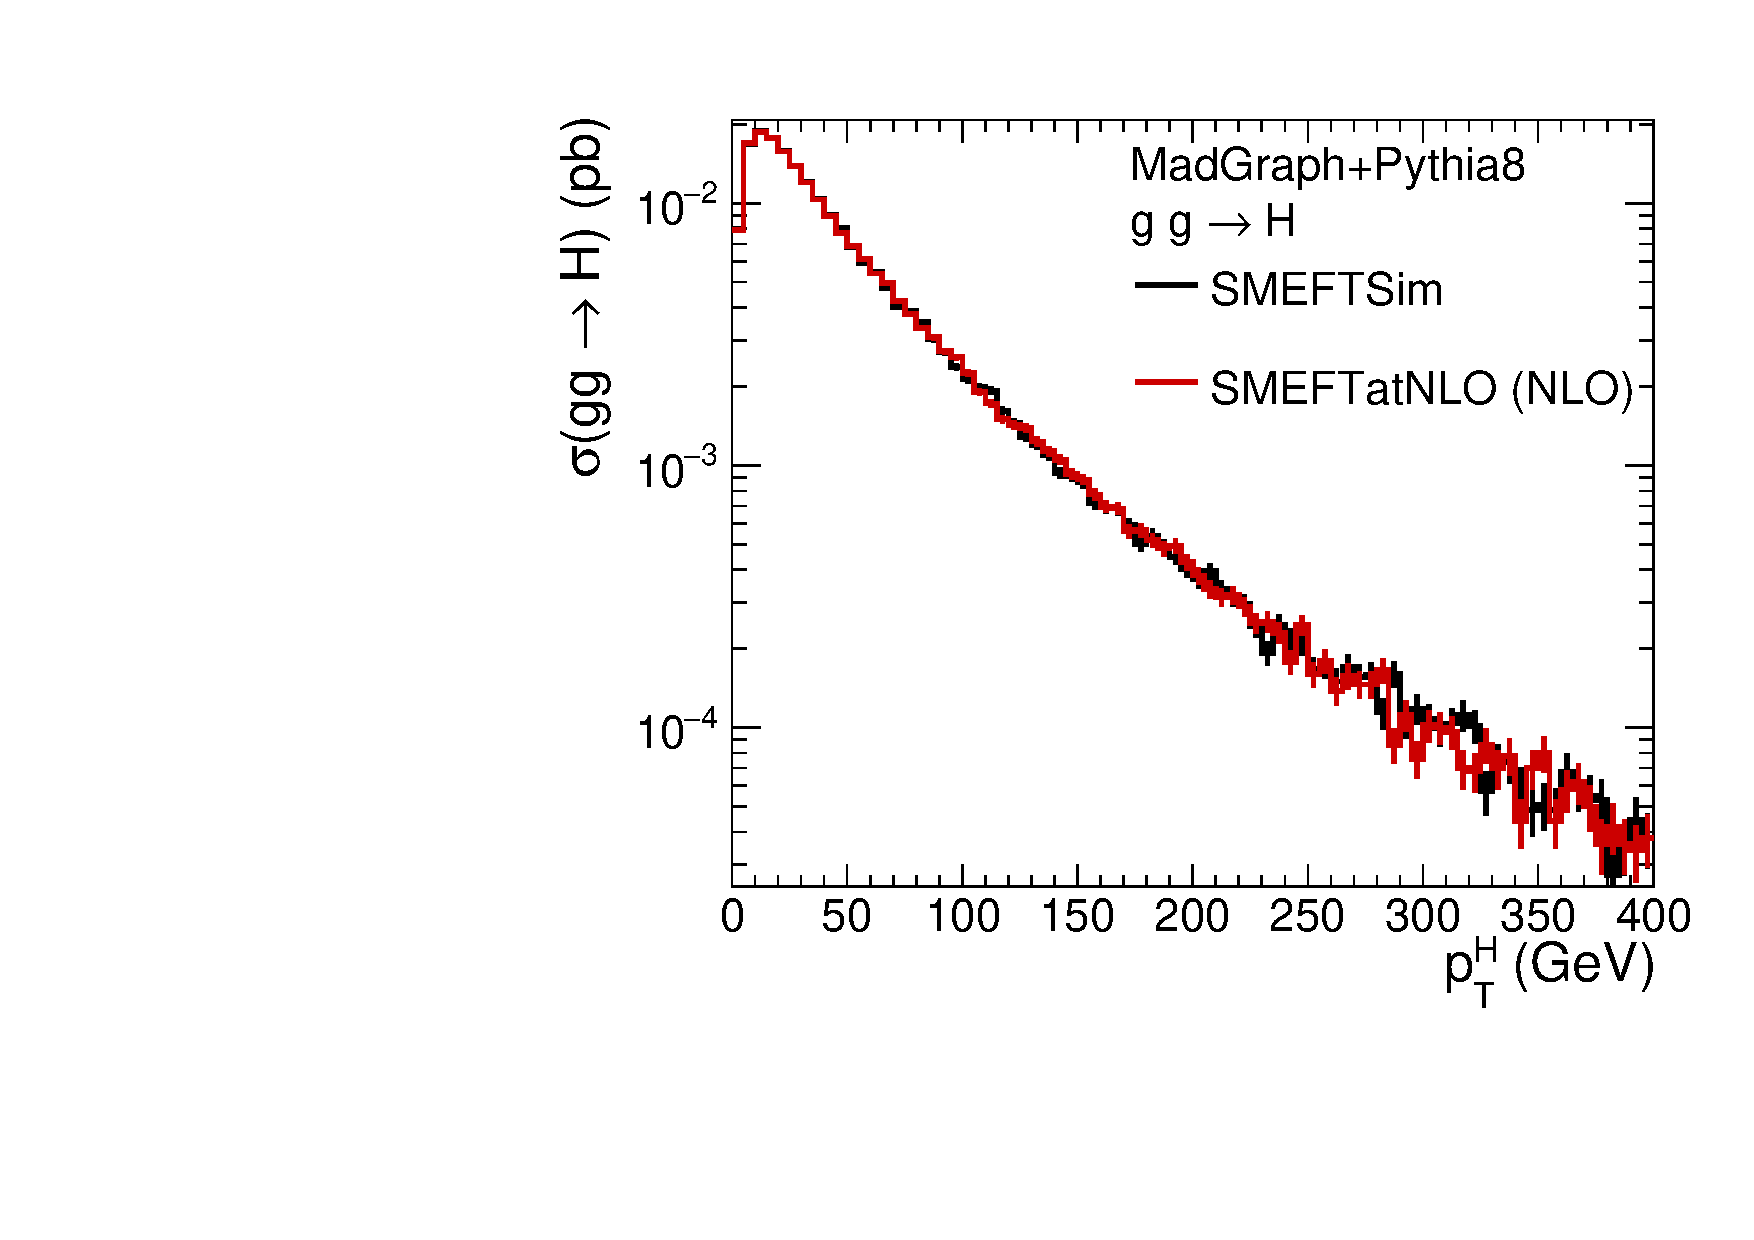
\includegraphics[width=0.49\linewidth]{figures/pT_Higgs.pdf}
  \begin{tikzpicture}[node distance=2cm and 0cm,scale=1.0]
      \coordinate[label=left:$g$] (q1) at (0,2);
      \coordinate[label=left:$g$] (q2) at (0,-2);
      \coordinate[] (V1) at (1,0);
      \coordinate[] (V2) at (3,0);
      \coordinate[] (V3) at (4.5,2);
      \coordinate[] (V4) at (4.5,0);
      \coordinate[] (V5) at (4.5,-2);
      \coordinate[label=right:$H$] (q3) at (6,2);
      \coordinate[label=right:$g$] (q4) at (6,0);
      \coordinate[label=right:$g$] (q5) at (6,-2);
      \draw[gluon] (q1) -- (V1);
      \draw[gluon] (q2) -- (V1);
      \draw[gluon] (V1) -- node[above]{$g$} (V2);
      \draw[particle] (V2) -- node[left]{$t$} (V3);
      \draw[particle] (V5) -- node[left]{$t$} (V2);
      \draw[particle] (V3) -- node[left]{$t$} (V4);
      \draw[particle] (V4) -- node[left]{$t$} (V5);
      \draw[scalar] (V3) -- (q3);
      \draw[gluon] (V4) -- (q4);
      \draw[gluon] (V5) -- (q5);

    \end{tikzpicture}    
    \caption{ Left: Comparison of the differential cross section of  $gg\to H$ as a function of $p_{\textrm T}^{ \textrm H}$ in \SMEFTsim\ and \SMEFTatNLO. Right: Example diagram contributing to $gg\to H +j$ which is not considered in \SMEFTsim\ but it is implemented in \SMEFTatNLO.}
    \label{fig:higgseft:diagram}
\end{figure}

\subsection{Summary and conclusions}
In the absence of hints for new physics in the LHC, the SMEFT approach started to be widely adopted by the experimental collaborations for the interpretation of their measurements. In order to be able to have predictions for the SMEFT, implementation of the SM plus dimension-6 Lagrangian in form of UFO files that can be interfaced with modern event generators are needed. Two different tools: \SMEFTsim\ and \SMEFTatNLO\ have been used and compare to study the $gg\to H$ and $gg\to ZH$ loop-induced processes. For the former, which is mainly meant for performing LO calculations, the $gg\to ZH$ process cannot be simulated and only one-loop functions for $gg\to H$ are implemented.
%It lacks, for example, of $gg\to Hg$ one loop-function exists making the calculation of Higgs plus jets unreliable. It also truncates the Lagrangian for contributions that have a loop suppression on top of the $\Lambda^{-2}$.

In this work we have compared both tools for the $pp\to t\bar{t}H$ and $pp\to ZH$ production processes. The agreement between the predictions for the SM and interference terms is excellent except for the $\mathcal{O}_{\textrm tG}$ operator. Some other operators like $\mathcal{O}_{\textrm tW}$, $\mathcal{O}_{\textrm tZ}$, or two-fermion currents involving quarks cannot be directly compared. Even if the definition of each operator is available in both models, it would be helpful for the user to to have a clear mapping operators in the different tools.

The SMEFT effects have been studied by means of the distortion of the SM prediction shape and normalisation in differential cross sections as well as the parametrisation of STXS bins. Only the interference effects have been investigated. For $gg\to H$, the operators \cpG\ and \ctG\ have a different effect compared with the SM when different scales are proven, increasing at higher energies.
The parametrisation in terms of STXS bins for $\mathcal{O}_{\psi G}$ differs from others that can be found in the literature using \SMEFTsim\ due to the differences in the implementation of this process in both tools. The \SMEFTatNLO\ tool is the only one that provides reliable description of the Higgs plus jets production in gluon-gluon fusion.

For $gg\to ZH$, with $Z\to l^{+}l^{-}$,  many operators change the cross sections. However, most of them just introduce a deviation in the normalisation of the SM predictions at the interference level without distorting the SM shape. Among the ones that have an energy dependence we can find: $\mathcal{O}_{tG}$, $\mathcal{O}_{t\psi}$ or $\mathcal{O}_{\psi q_i}^{(3)}$ 

The NLO effects on the decays have not been studied here. This work could have been extended with studies of $H\to \gamma\gamma$ and $ H\to Z\gamma$. They exist in the literature~\cite{Dawson:2018liq,Dedes:2018seb} for $H\to \gamma\gamma$. However, none of the tools are able to provide the NLO QED corrections for these processes in the SMEFT.



~\newline~

%= undefine macros (MANDATORY) ====================
\let\Herwig\undefined
\let\Pythia\undefined
\let\Sherpa\undefined
\let\Rivet\undefined
\let\Professor\undefined
\let\eps\undefined
\let\mc\undefined
\let\mr\undefined
\let\mb\undefined
\let\tm\undefined




